\documentclass[russian,english]{llncs}
\usepackage[utf8]{inputenc}
\usepackage[T2A]{fontenc}
\usepackage[final]{graphicx}
\usepackage{epstopdf}
\usepackage[labelsep=period]{caption}
\usepackage[hyphens]{url}
\usepackage{amssymb,amsmath,mathrsfs}
\usepackage[russian,english]{babel}
%\usepackage{multicol}
\usepackage[ruled,vlined,linesnumbered,algo2e]{algorithm2e}
%\usepackage{algorithm}
%\usepackage[noend]{algorithmic}
\usepackage{color}
\usepackage{cmap}
\usepackage{array}

\tolerance=1000
\hbadness=5000
\newcommand{\const}{\mathrm{const}}
\newcommand{\tsum}{\mathop{\textstyle\sum}\limits}
\newcommand{\tprod}{\mathop{\textstyle\prod}\limits}
\newcommand{\cov}{\mathop{\rm cov}\limits}
\newcommand{\Dir}{\mathop{\rm Dir}\nolimits}
\newcommand{\norm}{\mathop{\rm norm}\limits}
\newcommand{\KL}{\mathop{\rm KL}\nolimits}
%\renewcommand{\geq}{\geqslant}
%\renewcommand{\leq}{\leqslant}
\newcommand{\eps}{\varepsilon}
\newcommand{\cond}{\mspace{3mu}{|}\mspace{3mu}}
\newcommand{\Loss}{\mathscr{L}}
\newcommand{\RR}{\mathbb{R}}
\newcommand{\cL}{\mathscr{L}}
\newcommand{\cP}{\mathscr{P}}
\newcommand{\kw}[1]{\mbox{\textsf{#1}}}
\SetKwFor{ForAll}{\textbf{for all}}{}{}

\begin{document}
%%Analysis of Images, Social Networks, and Texts
\title{
    Parallel Non-blocking Deterministic Algorithm for Online Topic Modeling
}
\author{
    Oleksandr Frei\inst{1}
    \and
    Murat Apishev\inst{2}
}
\institute{\noindent
    Moscow Institute of Physics and Technology, Moscow, Russia,
    ~~\email{oleksandr.frei@gmail.com}
    \and
    National Research University Higher School of Economics, Moscow, Russia, \\
    ~~\email{great-mel@yandex.ru}
}

\maketitle

\begin{abstract}
In this paper we present a new asynchronous algorithm for learning additively regularized topic models
and discuss the main architectural details of our implementation.
The key property of the new algorithm is that it behaves in a fully deterministic fashion,
which is typically hard to achieve in a non-blocking parallel implementation. The algorithm
had been
recently implemented in the BigARTM library (\texttt{http://bigartm.org}).
Our new algorithm is compatible with all features previously introduced in BigARTM library,
including multimodality, regularizers and scores calculation.
While the existing BigARTM implementation compares favorably
with alternative packages such as Vowpal Wabbit or Gensim,
the new algorithm brings further improvements in CPU utilization,
memory usage, and spends even less time to achieve the same perplexity.

\vspace{1em}
\textbf{Keywords:}
    probabilistic topic modeling,
    additive regularization of topic models,
    stochastic matrix factorization,
    EM-algorithm,
    online learning,
    asynchronous and parallel computing,
    BigARTM.
\end{abstract}

\section{Introduction}
%
%\cite{li13parserver}

Topic modeling~\cite{blei12ptm} is a powerful machine learning tool for statistical text analysis
that has been widely used in text mining, information retrieval, network analysis and other areas~\cite{daud10knowledge}.
Today a lot of research efforts around topic models are devoted to distributed implementations of
\emph{Latent Dirichlet Allocation} (LDA)~\cite{blei03latent},
a specific Bayesian topic model that uses Dirichlet conjugate prior.
This lead to numerous implementations such as
AD-LDA~\cite{newman09distributed}, PLDA~\cite{wang09plda} and PLDA{+}~\cite{liu11plda},
all designed to run on a big cluster.
Topic models of web scale can reach millions of topics and words,
yielding Big Data models with trillions of parameters~\cite{yuan15lightlda}.
Yet not all researchers and applications are dealing with so large web-scale collections.
Some of them require an efficient implementation that can run on a powerful workstation or even a laptop.
Such implementations are very useful,
as shown by the popular open-source packages
Vowpal Wabbit~\cite{langford07vw}, Gensim~\cite{rehurek10software} and Mallet~\cite{McCallum02mallet},
which are neither distributed nor sometimes even multi-threaded.

A similar optimization problem and its distributed implementations exist
in the Deep Neural Network area, as
DNN and Topic modeling both use Stochastic Gradient Descent (SGD) optimization.
The asynchronous SGD~\cite{dean2012sgd} does not directly apply to Topic modeling because
it is computationally less efficient to partition a topic model across nodes.
Limited parallelizability~\cite{seide2014sgd} of speech DNNs across nodes justify our focus on single-node optimizations.
However, scaling down a distributed algorithm can be challenging.
LightLDA~\cite{yuan15lightlda} is a major step in this direction,
however it focuses only on the LDA model.
Our goal is to develop a flexible framework that can learn a wide variety of topic models.

BigARTM~\cite{vfardi15aist} is an open-source library for
regularized multimodal topic modeling of large collections.
BigARTM is based on a novel technique of additive regularized topic models (ARTM)~\cite{voron14dan-eng,voron15mlj,voron15nonbayesian},
which gives a flexible multi-criteria approach to probabilistic topic modeling.
ARTM includes all popular models such as 
LDA~\cite{blei03latent}, 
PLSA~\cite{hofmann99plsi},
and many others.
Key feature of ARTM is that it provides a cohesive framework that allows users to combine
different topic models that previously did not fit together.

BigARTM is proven to be very fast compared to the alternative packages.
According to~\cite{vfardi15aist}, BigARTM
runs approx. $10$ times faster compared to Gensim~\cite{rehurek10software}
and twice as fast as
Vowpal Wabbit~\cite{langford07vw}
in a single thread.
With multiple threads BigARTM wins even more
as it scales linearly up to at least 16 threads.
In this paper we address the remaining limitations of the library,
including performance bottlenecks
and non-deterministic behavior of the Online algorithm.

%Deterministic behavior is an important property for any algorithm,
%including those of a stochastic nature.
%For the end users of a software system run-to-run reproducibility is a must-have property,
%because this is what they expect based on their previous experience.
%Indeed, refreshing a web-pages or re-doing an operation tend to
%produce an identical result, regardless of how much software complexity is hidden behind the scenes.
%For the researches determinism is also important
%because it enables them to reproduce their old experiments
%and study impact of various parameters on the result.
%Finally, for the developers of the algorithm
%determinism allow to reproduce bugs and write simple unit-tests with well-defined results.

%Determinism is particularly hard to achieve
%in concurrent implementations, because in a multi-threaded environment
%it might not be sufficient to just fix a random seed or an initial approximation.
%In this paper we present a deterministic modification of parallel non-blocking algorithm
%for online topic modeling, previously developed for BigARTM library.
%We implement new algorithm in BigARTM and demonstrate that new version converges faster
%than previous algorithm in terms of perplexity,
%yet being more efficient in CPU and memory usage.

The rest of the paper is organized as follows.
Section~\ref{sec:Notation}
introduces basic notation.
Sections~\ref{sec:OfflineARTM} and \ref{sec:OnlineARTM}
summarize offline and online algorithms for learning ARTM models.
Sections~\ref{sec:AsyncARTM} and \ref{sec:DetAsyncARTM}
discuss asynchronous modifications of the online algorithm.
Section~\ref{sec:Architecture}
compares BigARTM architecture between versions~\kw{0.6} and~\kw{0.7}.
Section~\ref{sec:Experiments}
reports the results of our experiments on large datasets.
Section~\ref{sec:Conclusions}
discusses advantages, limitations and open problems of BigARTM.

%sashafrey:
%really technical topics in my opinion does not belong to AISTconf article;
%it would be more appropriate to discuss the following in the full 12-page article in http://www.ispras.ru/en/ journal
%\begin{itemize}
%    \item Details of CLI interface and python interface, usage examples
%    \item List new features: coherence score and regularizer, classification, documents markdown (aka $p_{tdw}$ matrices)
%    \item Our technologies (Protobuf for low-level C API, Boost Serialize for import/export, GLog, GFlags, GTest, etc)
%    \item Our build solution and CI solution (CMake, Visual Studio, GitHub, Git submodules, Travis, Apveyour, Read-The-Docs)
%    \item Why people care about run-to-run reproducibility
%    https://software.intel.com/en-us/articles/consistency-of-floating-point-results-using-the-intel-compiler
%\end{itemize}

\section{Notation}
\label{sec:Notation}

Let
$D$ denote a finite set (collection) of texts and
$W$ denote a~finite set (vocabulary) of all words from these texts.
Let
$n_{dw}$ denote the number of occurrences of a word $w \in W$ in a document $d \in D$;
$n_{dw}$ values form a sparse matrix of size~$|W| \times |D|$,
known as \emph{bag-of-words} representation of the collection.

Given an $(n_{dw})$ matrix, a probabilistic topic model finds two matrices:
$\Phi~=~(\phi_{wt})$ and $\Theta = (\theta_{td})$,
of sizes $|W| \times |T|$ and $|T| \times |D|$ respectively,
where $|T|$ is a user-defined number of \emph{topics} in the model (typically $|T| << |W|$).
Matrices~$\Phi$ and $\Theta$
provide a compressed representation of the $(n_{dw})$ matrix:
\[
n_{dw} \approx n_d \sum_{t \in T} \phi_{wt} \theta_{td}, \text { for all } d \in D, w \in W,
\]
where $n_d = \sum_{w \in W} n_{dw}$ denotes the total number of words in a document $d$.

To learn $\Phi$ and $\Theta$ from $(n_{dw})$ an additively-regularized topic model (ARTM) maximizes
the log-likelihood, regularized via an additional penalty term $R(\Phi, \Theta)$:
\begin{gather}
\label{eq:ARTM}
    F(\Phi, \Theta) = \sum_{d\in D}\sum_{w\in W} n_{dw} \ln \sum_{t\in T} \phi_{wt} \theta_{td} + R(\Phi, \Theta)
    \;\to\; \max_{\Phi,\Theta}.
\end{gather}
Regularization penalty $R(\Phi, \Theta)$ may incorporate external knowledge
of the expert about the collection.
With no regularization (${R=0}$) it corresponds to PLSA~\cite{hofmann99plsi}.
Many Bayesian topic models, including LDA~\cite{blei03latent}, can be represented
as special cases of ARTM with different regularizers~$R$,
as shown in~\cite{voron15mlj}.

In~\cite{voron14dan-eng} it is shown that the \mbox{local} maximum $(\Phi,\Theta)$
of problem~\eqref{eq:ARTM} satisfies
the following system of equations:
\begin{align}
    \label{eq:Estep}
    p_{tdw} &= \norm_{t\in T} \bigl(\phi_{wt}\theta_{td}\bigr);
\\
    \label{eq:Mstep:phi}
    \phi_{wt} &= \norm_{w\in W}
        \biggl(
            n_{wt} + \phi_{wt} \frac{\partial R}{\partial \phi_{wt}}
        \biggr);
        \quad
            n_{wt} = \sum_{d\in D} n_{dw} p_{tdw};
%    \phi_{wt} &= \norm_{w\in W}
%        \biggl(
%            n_{wt} + r_{wt}
%        \biggr);
%    \quad
%    n_{wt} = \sum_{d\in D} n_{dw} p_{tdw};
%    \quad
%    r_{wt} = \phi_{wt} \frac{\partial R}{\partial \phi_{wt}};
\\
    \label{eq:Mstep:theta}
    \theta_{td} &= \norm_{t\in T}
        \biggl(
            n_{td} + \theta_{td} \frac{\partial R}{\partial \theta_{td}}
        \biggr);
        \quad\quad
            n_{td} = \sum_{w\in d} n_{dw} p_{tdw};
%    \theta_{td} &= \norm_{t\in T}
%        \biggl(
%            n_{td} + r_{td}
%        \biggr);
%    \quad
%    r_{td} = \theta_{td} \frac{\partial R}{\partial \theta_{td}};
        %\sum_{m=1}^M \tau_m \!\!\sum_{w\in W^m}\!\!\! n_{dw} p_{tdw};
\end{align}
where operator
$\norm_{i \in I} x_i = \frac{\max\{x_i,0\}}{\sum\limits_{j\in I} \max\{x_j,0\}}$
transforms a~vector $(x_i)_{i \in I}$ to a~discrete distribution,
$n_{wt}$ counters represent term frequency of word $w$ in topic $t$.
% Hard to make up a similar explanation for $n_{td}$. Thesse counters represent "document frequency"? No...

Learning of $\Phi$ and $\Theta$ from \eqref{eq:Estep}--\eqref{eq:Mstep:theta} can be done by EM-algorithm,
which starts from random values in $\Phi$ and $\Theta$, and iterates
E-step \eqref{eq:Estep} and
M-steps \eqref{eq:Mstep:phi},\eqref{eq:Mstep:theta}
until convergence.
% Simple-iteration method - skip for now
In the sequel we discuss several variations of such EM-algorithm,
which are all based on the above formulas but differ in the way how operations are ordered and grouped together.

In addition to plain text, many collections have other metadata,
such as authors, class or category labels, date-time stamps,
or even associated images, audio or video clips, usage data, etc.
In~\cite{voron15nonbayesian} this data was represented as \emph{modalities},
where the overall vocabulary $W$ is partitioned into $M$ subsets
$W = W^1 \sqcup \dots \sqcup W^M$, one subset per modality,
and in \eqref{eq:Mstep:phi} matrix $\Phi$ is normalized independently 
within each modality.
Incorporating modalities into a topic model improves its quality
and makes it applicable for classification, cross-modal retrieval, or making recommendations.
In the sequel we list all algorithms for one modality,
but our implementation in BigARTM supports the general case.

\section{Offline Algorithm}
\label{sec:OfflineARTM}

\SetAlgoSkip{}
\begin{algorithm2e}[t]
	\caption{\kw{ProcessDocument}($d, \Phi$)}
	\label{alg:ProcessDocument}
	\BlankLine
	\KwIn{document $d \in D$, matrix $\Phi=(\phi_{wt})$;}
	\KwOut{matrix $(\tilde n_{wt})$, vector $(\theta_{td})$ for the document $d$;}
	\BlankLine
	initialize $\theta_{td} := \frac{1}{|T|}$ for all $t \in T$\;
	\Repeat{$\theta_d$ {\upshape converges}}{
		\label{alg:ProcessDocument:innerLoopBegin}
		$p_{tdw} := \norm_{t\in T} \bigl(\phi_{wt}\theta_{td}\bigr)$ for all $w\in d$ and $t \in T$\;
		$\theta_{td} := \norm_{t\in T}
		\bigl(
		\sum_{w\in d} n_{dw} p_{tdw} + \theta_{td} \frac{\partial R}{\partial \theta_{td}}
		\bigr)$ for all $t \in T$\;
	}
	\label{alg:ProcessDocument:innerLoopEnd}
	$\tilde n_{wt} := n_{dw} p_{tdw}$ for all $w \in d$ and $t \in T$\;
\end{algorithm2e}
\begin{algorithm2e}[t]
\caption{Offline ARTM}
\label{alg:OfflineARTM}
\BlankLine
\KwIn{collection $D$;}
\KwOut{matrix $\Phi = (\phi_{wt})$;}
\BlankLine
initialize $(\phi_{wt})$\;
create batches $D := D_1 \sqcup D_2 \sqcup \dots \sqcup D_B$\;
\label{alg:OfflineARTM:FormBatches}
\Repeat{$(\phi_{wt})$ {\upshape converges}}{
    %$\tilde n_{wt} := 0$ for all $w \in W$ and $t \in T$\;
    %\ForAll{documents $d \in D$} {
    %    $(\tilde n_{wt}) := (\tilde n_{wt}) + \kw{ProcessDocument}(d, \Phi)$\;
    %}
    \label{alg:OfflineARTM:Accumulate}
    $(n_{wt}) := \mathlarger\sum\limits_{b=1, \dots, B} \; \mathlarger\sum\limits_{d \in D_b} \; \kw{ProcessDocument}(d, \Phi)$\;
    \label{alg:OfflineARTM:Normalize}
    $(\phi_{wt}) := \norm_{w \in W} (n_{wt} + \phi_{wt} \frac{\partial R}{\partial \phi_{wt}})$\;
}
\end{algorithm2e}

\begin{figure}[t]
\centering
\begin{tabular}{c}
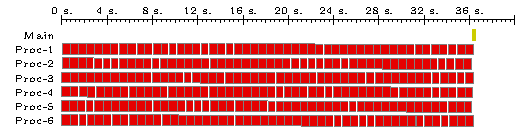
\includegraphics[height=4cm, width=12cm]{plots/offline.pdf} \\
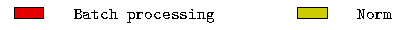
\includegraphics[scale=1]{plots/legend_offline.pdf}
\end{tabular}
\caption{Gantt chart for \kw{Offline ARTM} (Alg. \ref{alg:OfflineARTM})} \label{fig:gantt:OfflineARTM}
\end{figure}

\kw{Offline ARTM} (Alg. \ref{alg:OfflineARTM}) relies on subroutine
\kw{ProcessDocument} (Alg. \ref{alg:ProcessDocument}),
which corresponds to equations \eqref{eq:Estep} and \eqref{eq:Mstep:theta}
from the solution of the ARTM optimization problem \eqref{eq:ARTM}.
\kw{ProcessDocument} requires a fixed $\Phi$ matrix
and a vector $n_{dw}$ of term frequencies for a given document $d \in D$,
and as a result it returns a topical distribution $(\theta_{td})$ for the document,
and a matrix $(\hat n_{wt})$ of size $|d| \times |T|$,
where~$|d|$ denotes the number of distinct words in the document.
\kw{ProcessDocument} might also be useful as a separate routine which finds $(\theta_{td})$ distribution for a new document,
but in the \kw{Offline} algorithm it is instead used as a building block in an iterative EM-algorithm that finds the $\Phi$ matrix.

\kw{Offline} algorithm performs scans over the collection, calling \kw{ProcessDocument}
for each document $d \in D$ from the collection,
and then aggregating the resulting~$(\hat n_{wt})$ matrices into the final $(n_{wt})$ matrix of size $|W| \times |T|$.
After each scan it recalculates $\Phi$ matrix according to the equation $\eqref{eq:Mstep:phi}$.

%To split collection into batches and process them concurrently is a common approach,
%introduced in AD-LDA algorithm~\cite{newman09distributed}, and
%then further developed in PLDA~\cite{wang09plda} and PLDA{+}~\cite{liu11plda} algorithms.

At step \ref{alg:OfflineARTM:FormBatches} we partition collection $D$ into batches $(D_b)$.
This step is not strictly necessary for \kw{Offline} algorithm,
but it rather reflects an internal implementation detail.
For performance reasons the outer loop over batches $b = 1, \dots, B$ is parallelized across multiple threads,
and within each batch the inner loop over documents~$d \in D_b$
is executed in a single thread.
Each batch is stored in a separate file on disk to allow out-of-core streaming of the collection.
For typical collections it is reasonable to have around $1000$ documents per batch,
however for ultimate performance we encourage users to experiment with this parameter.
Too small batches can cause disk IO overhead due to lots of small reads,
while too large batches will result in bigger tasks that will not be distributed evenly across computation threads.

Note that $\theta_{td}$ values appear only within $\kw{ProcessDocument}$ subroutine.
This leads to efficient memory usage because the implementation never stores the entire theta matrix $\Theta$ at any given time.
Instead, $\theta_{td}$ values are recalculated from scratch on every pass through the collection.

Fig. \ref{fig:gantt:OfflineARTM} shows a Gantt chart of the \kw{Offline} algorithm.
Here and in the sequel Gantt charts are built for a single EM-iteration on
\kw{NYTimes} dataset\footnote{\url{https://archive.ics.uci.edu/ml/datasets/Bag+of+Words}}
($|D|=300$K, $|W|=102$K) with $|T|=16$ topics.
\kw{ProcessBatch} boxes corresponds to the time spent in processing an individual batch.
The final box \kw{Norm}, executed on the main thread,
correspond to the time spent in the step \ref{alg:OfflineARTM:Normalize} in Alg. \ref{alg:OfflineARTM}
where $n_{wt}$ counters are normalized to produce a new $\Phi$ matrix.


\section{Online Algorithm}
\label{sec:OnlineARTM}

\kw{Online ARTM} (Alg. \ref{alg:OnlineARTM}) generalizes
the Online variational Bayes algorithm,
suggested in~\cite{hoffman10online} for the LDA model.
\kw{Online ARTM} improves the convergence rate of the \kw{Offline ARTM}
by re-calculating matrix $\Phi$ each time after processing a certain number of batches.
To simplify the notation
we introduce a trivial subroutine
\[
\kw{ProcessBatches}(\{D_b\}, \Phi) = \mathlarger\sum\limits_{D_b} \mathlarger\sum\limits_{d \in D_b} \; \kw{ProcessDocument}(d, \Phi) \\
\]
that aggregates the output of $\kw{ProcessDocument}$ across a given set of batches at a constant $\Phi$ matrix.
Here the partition of the collection $D := D_1 \sqcup D_2 \sqcup \dots \sqcup D_B$
into batches
plays a far more significant role than in the \kw{Offline} algorithm,
because different partitioning algorithmically affects the result.
At step \ref{alg:OnlineARTM:Merge} the new $n_{wt}^{i+1}$ values are calculated as a convex combination
of the old values $n_{wt}^{i}$ and the value $\hat n_{wt}^{i}$ produced on the recent batches.
Old counters $n_{wt}^{i}$ are scaled by a factor $(1 - \rho_i)$,
which depends on the iteration number. A common strategy is to use $\rho_i = (\tau_0 + i)^{-\kappa}$,
where typical values for $\tau_0$ are between $64$ and $1024$, for $\kappa$ --- between $0.5$ and $0.7$.

\SetAlgoSkip{}
\begin{algorithm2e}[t]
	\caption{Online ARTM} %\mbox{regularized} topic modeling
	\label{alg:OnlineARTM}
	\BlankLine
	\KwIn{collection $D$, parameters $\eta, \tau_0, \kappa$;}
	\KwOut{matrix $\Phi = (\phi_{wt})$;}
	\BlankLine
	create batches $D := D_1 \sqcup D_2 \sqcup \dots \sqcup D_B$\;
	initialize $(\phi^0_{wt})$\;
	\For{$i = 1, \dots, \lfloor B / \eta \rfloor$} {
		$(\hat n^i_{wt}) := \kw{ProcessBatches}(\{D_{\eta (i - 1) + 1}, \dots, D_{\eta i}\}, \Phi^{i - 1})$\;
		\label{alg:OnlineARTM:ProcessBatches}
		$\rho_i := (\tau_0 + i)^{-\kappa}$\;
		\label{alg:OnlineARTM:Rho}
		$(n^{i}_{wt}) := (1 - \rho_i) \cdot (n^{i-1}_{wt}) + \rho_i \cdot (\hat n^{i}_{wt})$\;
		\label{alg:OnlineARTM:Merge}
		$(\phi^{i}_{wt}) := \norm_{w \in W} (n^{i}_{wt} + \phi^{i - 1}_{wt} \frac{\partial R}{\partial \phi_{wt}})$\;
		\label{alg:OnlineARTM:Normalize}
	}
\end{algorithm2e}
\begin{figure}[t!]
	\centering
	\begin{tabular}{c}
		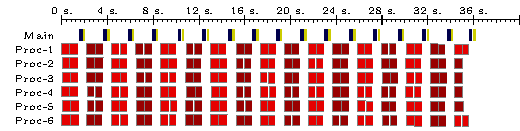
\includegraphics[height=4cm, width=12cm]{plots/online.pdf} \\
		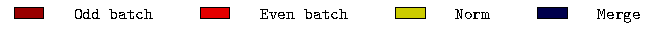
\includegraphics[scale=1]{plots/legend_online.pdf}
	\end{tabular}
	\caption{Gantt chart for \kw{Online ARTM} (Alg. \ref{alg:OnlineARTM})} \label{fig:gantt:OnlineARTM}
\end{figure}

As in the \kw{Offline} algorithm, the outer loop over batches
$D_{\eta (i - 1) + 1}, \dots, D_{\eta i}$ is executed concurrently across multiple threads.
The problem with this approach is that none of the threads have any useful work to do during steps
\ref{alg:OnlineARTM:Rho}-\ref{alg:OnlineARTM:Normalize} of the \kw{Online} algorithm.
The threads can not start processing the next batches because a new version of $\Phi$ matrix is not ready yet.
As a result the CPU utilization stays low, and the run-time Gantt chart of the \kw{Online} algorithm typically looks like in Fig. \ref{fig:gantt:OnlineARTM}.
Boxes \kw{Even batch} and \kw{Odd batch} both correspond to step \ref{alg:OnlineARTM:ProcessBatches},
and indicate the version of the $\Phi^i$ matrix (even $i$ or odd $i$).
\kw{Merge} correspond to the time spent merging $n_{wt}$ with $\hat n_{wt}$.
\kw{Norm} is, as before, the time spent normalizing $n_{wt}$ counters into the new $\Phi$ matrix.

In the next two sections we present asynchronous modifications of the online algorithm that result in better CPU utilization.
The first of them (\kw{Async~ARTM}) has non-deterministic behavior and few performance bottlenecks.
The second algorithm (\kw{DetAsync~ARTM}) addresses these problems.

\section{Async: Asynchronous Online Algorithm}
\label{sec:AsyncARTM}

\begin{figure}[h]
	\centering
	\begin{tabular}{c}
		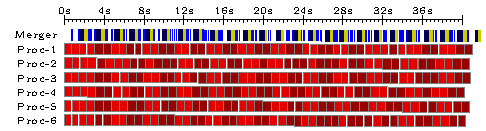
\includegraphics[height=4cm, width=12cm]{plots/old.pdf} \\
		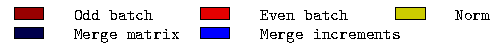
\includegraphics[scale=1]{plots/legend_old.pdf}
	\end{tabular}
	\caption{Gantt chart for \kw{Async ARTM} from \kw{BigARTM v0.6} --- normal execution} \label{fig:gantt:AsyncARTM}
\end{figure}

\begin{figure}[h]
	\centering
	\begin{tabular}{c}
		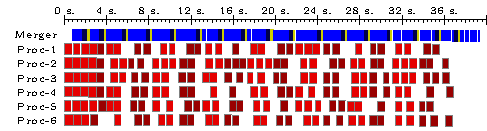
\includegraphics[height=4cm, width=12cm]{plots/old_slow.pdf} \\
		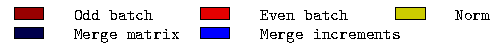
\includegraphics[scale=1]{plots/legend_old.pdf}
	\end{tabular}
	\caption{Gantt chart for \kw{Async ARTM} from \kw{BigARTM v0.6} --- performance issues} \label{fig:gantt:AsyncARTM:slow}
\end{figure}

\kw{Async} algorithm was implemented in \kw{BigARTM v0.6} as described in~\cite{vfardi15aist}.
The idea is to trigger asynchronous execution of the \kw{Offline} algorithm
and store the resulting $\hat n_{wt}$ matrices into a queue.
Then, whenever the number of elements in the queue becomes equal to $\eta$,
the \kw{Async} algorithm performs steps \ref{alg:OnlineARTM:Rho}-\ref{alg:OnlineARTM:Normalize}
of the \kw{Online ARTM} (Alg. \ref{alg:OnlineARTM}).
For performance reasons merging of the $\hat n_{wt}$ counters happens in a background by a dedicated \emph{Merger} thread.

First problem of the \kw{Async} algorithm is that it does not define the order
in which $\hat n_{wt}$ are merged.
This order is usually different from the original order of the batches,
and typically it changes from run to run.
This affects the final $\Phi$ matrix which also changes from run to run.

Another issue with \kw{Async} algorithm is that
queuing $\hat n_{wt}$ counters may considerably increase the memory usage,
and also lead to performance bottlenecks in the \emph{Merger} thread.
In some cases the execution of the \kw{Async} algorithm is
as efficient as for the \kw{Offline} algorithm,
as shown on Fig. \ref{fig:gantt:AsyncARTM}.
However, certain combination of the parameters
(particularly, small batch size or small number of iterations in \kw{ProcessDocument}'s inner loop 
\ref{alg:ProcessDocument:innerLoopBegin}-\ref{alg:ProcessDocument:innerLoopEnd})
might overload the merger thread.
Then the Gantt chart may look as on Fig. \ref{fig:gantt:AsyncARTM:slow},
where most threads are waiting because there is no space left in the queue
to place $n_{wt}$ counters.

In the next section we resolve the aforementioned problems
by introducing a new \kw{DetAsync} algorithm,
which has an entirely deterministic behavior
and achieves high CPU utilization without requiring user to tweak the parameters.

\section{DetAsync: Deterministic Async Online Algorithm}
\label{sec:DetAsyncARTM}

\SetAlgoSkip{}
\begin{algorithm2e}[t]
	\caption{DetAsync ARTM} %\mbox{regularized} topic modeling
	\label{alg:DetAsyncARTM}
	\BlankLine
	\KwIn{collection $D$, parameters $\eta, \tau_0, \kappa$;}
	\KwOut{matrix $\Phi = (\phi_{wt})$;}
	\BlankLine
	create batches $D := D_1 \sqcup D_2 \sqcup \dots \sqcup D_B$\;
	initialize $(\phi^0_{wt})$\;
	$F^1 := \kw{AsyncProcessBatches}(\{D_{1}, \dots, D_{\eta}\}, \Phi^0)$\;
	\label{alg:DetAsyncARTM:FirstStep}
	\For{$i = 1, \dots, \lfloor B / \eta \rfloor$} {
		\If{$i \neq \lfloor B / \eta \rfloor$}{
			\label{alg:DetAsyncARTM:IfStatement}
			$F^{i+1} := \kw{AsyncProcessBatches}(\{D_{\eta i + 1}, \dots, D_{\eta i + \eta}\}, \Phi^{i-1})$\;
		}
		$(\hat n^i_{wt}) := \kw{Await}(F^i)$\;
		$\rho_i := (\tau_0 + i)^{-\kappa}$\;
		$(n^{i}_{wt}) := (1 - \rho_i) \cdot (n^{i-1}_{wt}) + \rho_i \cdot (\hat n^{i}_{wt})$\;
		$(\phi^{i}_{wt}) := \norm_{w \in W} (n^{i}_{wt} + \phi^{i-1}_{wt} \frac{\partial R}{\partial \phi_{wt}})$\;
	}
\end{algorithm2e}

\begin{figure}[t]
	\centering
	\begin{tabular}{c}
		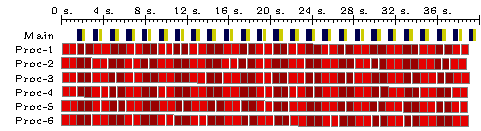
\includegraphics[height=4cm, width=12cm]{plots/async.pdf} \\
		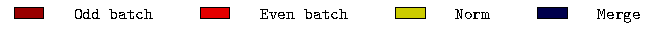
\includegraphics[scale=1]{plots/legend_online.pdf}
	\end{tabular}
	\caption{Gantt chart for \kw{DetAsync ARTM} (Alg. \ref{alg:DetAsyncARTM})} \label{fig:gantt:DetAsyncARTM}
\end{figure}

\kw{DetAsync ARTM} (Alg. \ref{alg:DetAsyncARTM}) is based on two new routines, \kw{AsyncProcessBatches} and \kw{Await}.
The former is equivalent to \kw{ProcessBatches}, except that it just queues the task for an asynchronous execution and returns immediately.
Its output is a future object (for example, an \kw{std::future} from \kw{C++11} standard),
which can be later passed to $\kw{Await}$ in order to get the actual result, e.g. in our case the $\hat n_{wt}$ values.
In between calls to \kw{AsyncProcessBatches} and \kw{Await} the algorithm
can perform some other useful work, while the background threads are calculating the $(\hat n_{wt})$ matrix.

To calculate $\hat n^{i+1}_{wt}$ it uses $\Phi^{i-1}$ matrix,
which is one generation older than $\Phi^{i}$ matrix used by the \kw{Online} algorithm.
This adds an extra ``offset'' between the moment when $\Phi$ matrix is calculated and the moment when it is used,
and as a result gives the algorithm additional flexibility to distribute more payload to computation threads.
Steps \ref{alg:DetAsyncARTM:FirstStep} and \ref{alg:DetAsyncARTM:IfStatement} of the algorithm
are just technical tricks to implement the ``offset'' idea.

Adding an ``offset'' should negatively impact the convergence of the \kw{DetAsync} algorithm
compared to the \kw{Online} algorithm.
For example, in \kw{AsyncProcessBatches} the initial matrix $\Phi^0$ is used twice,
and the two last matrices $\Phi^{\lfloor B / \eta \rfloor - 1}$ and $\Phi^{\lfloor B / \eta \rfloor}$ will not be used at all.
%(except for $\Phi^{\lfloor B / \eta \rfloor}$ which forms the final result of the algorithm).
On the other hand the asynchronous algorithm gives better CPU utilization,
as clearly shown by the Gantt chart from Fig. \ref{fig:gantt:DetAsyncARTM}.
%The color scheme for the boxes is as in Fig. \ref{fig:gantt:DetAsyncARTM}.
This tradeoff between convergence and CPU utilization will be evaluated in section~\ref{sec:Experiments}.

\section{Implementation}
\label{sec:Architecture}

\begin{figure}[t]
	\begin{centering}
		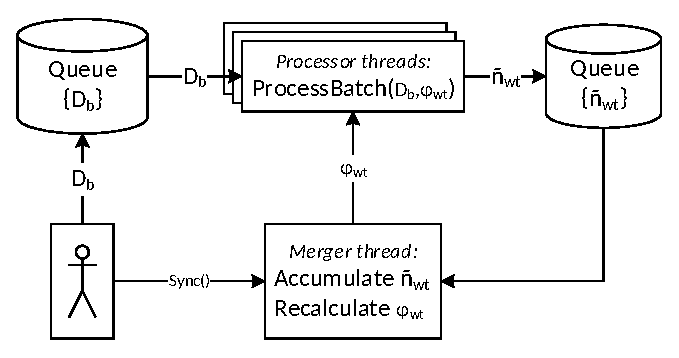
\includegraphics[height=40mm]{diagramm_artm_core.eps}
		\caption{Diagram of BigARTM components (old architecture)}
		\label{fig:diagramm_artm_core}
	\end{centering}
\end{figure}
\begin{figure}[t]
	\begin{centering}
		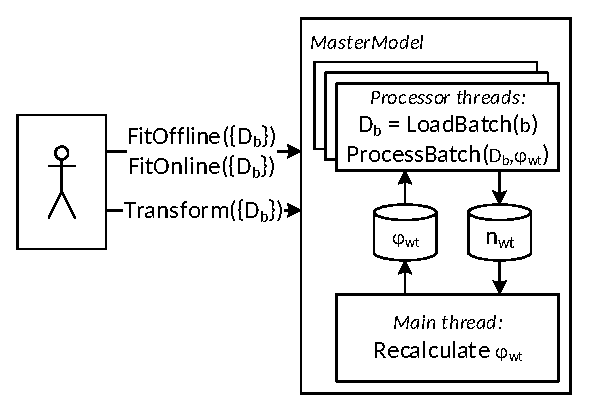
\includegraphics[height=47mm]{diagramm_artm_core_v07.eps}
		\caption{Diagram of BigARTM components (new architecture)}
		\label{fig:diagramm_artm_core_v07}
	\end{centering}
\end{figure}

The challenging part for the implementation is to aggregate the $\hat n_{wt}$ matrices across multiple batches,
given that they are processed in different threads.
The way BigARTM solves this challenge was changed between versions \kw{v0.6} (Fig. \ref{fig:diagramm_artm_core})
and \kw{v0.7} (Fig. \ref{fig:diagramm_artm_core_v07}).

In the old architecture the $\hat n_{wt}$ matrices were stored in a queue,
and then aggregated by a dedicated \emph{Merger thread}.
In the new architecture we removed Merger thread,
and $\hat n_{wt}$ are written directly into the final $n_{wt}$ matrix
concurrently from all processor threads.
To synchronize the write access we require that
no threads simultaneously update the same row in $\hat n_{wt}$ matrix,
yet the data for distinct words can be written in parallel.
This is enforced by spin locks $l_w$, one per each word in the vocabulary $W$.
At the end of \kw{ProcessDocument} we loop through all $w \in d$, acquire the corresponding lock $l_w$, append $\hat n_{wt}$ to $n_{wt}$ and release the lock.
This approach is similar to~\cite{smola10architecture},
where the same pattern is used to update a shared stated in a distributed topic modeling architecture.

In our new architecture we also removed \emph{DataLoader} thread, which previously was loading batches from disk.
Now this happens directly from processor thread, which simplified the architecture without sacrificing performance.

In addition, we provided a cleaner API so now the users may use simple \kw{FitOffline}, \kw{FitOnline} methods to learn the model,
and $\kw{Transform}$ to apply the model to the data.
Previously the users had to interact with low-level building blocks, such as \kw{ProcessBatches} routine.

\section{Experiments}
\label{sec:Experiments}


\begin{figure}[t]
	\centering
	\begin{minipage}[b]{0.4\textwidth}
		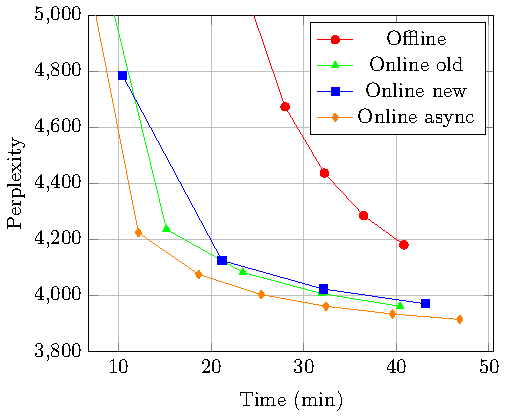
\includegraphics[scale=0.65]{plots/perplexity_time_plot_12.pdf}
	\end{minipage}
	$\qquad\quad$
	\begin{minipage}[b]{0.4\textwidth}
		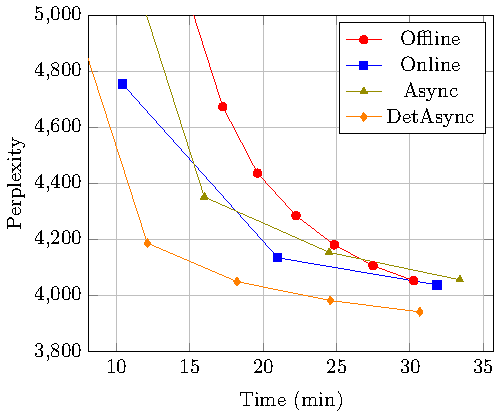
\includegraphics[scale=0.65]{plots/perplexity_time_plot_16.pdf}
	\end{minipage}
	\caption{Perplexity versus time for Pubmed (left) and Wikipedia (right), $|T| = 100$ topics}
	\label{fig:perf}
\end{figure}
\begin{table}[t]
	\caption{
		BigARTM peak memory usage, GB
	}
	\label{tab:memory}
	\centering\tabcolsep=4.3pt
	\begin{tabular}[t]{|l|ccccc|}
		\hline
		& $|T|$ & Offline   & Online    & DetAsync     & Async (\kw{v0.6})  \\
		\hline
		Pubmed & {1000}	& {5.17}   	& {4.68}   	& {8.18}   	& {13.4}      \\
		Pubmed & {100}	& {1.86}   	& {1.62}   	& {2.17}   	& {3.71}      \\
		Wiki   & {1000}	& {1.74}   	& {2.44}   	& {3.93}   	& {7.9}       \\ 
		Wiki   & {100}	& {0.54}   	& {0.53}   	& {0.83}   	& {1.28}       \\ 
		\hline
	\end{tabular}
\end{table}

In this section we compare the effectiveness of
\kw{Offline} (Alg. \ref{alg:OfflineARTM}),
\kw{Online} (Alg. \ref{alg:OnlineARTM}),
\kw{Async}~\cite{vfardi15aist} and
\kw{DetAsync} (Alg. \ref{alg:DetAsyncARTM}) algorithms.
According to~\cite{vfardi15aist} \kw{Async} algorithm
runs approx. $10$ times faster compared to Gensim~\cite{rehurek10software},
and twice as fast compared to
Vowpal Wabbit (VW)~\cite{langford07vw}
in a single thread;
and with multiple threads BigARTM wins even more.

In the experiments we use \emph{Wikipedia} dataset ($|D| = 3.7$M articles, $|W| = 100$K words)
and \emph{Pubmed} dataset ($|D| = 8.2$M abstracts, $|W| = 141$K words).
The experiments were run on Intel Xeon CPU E5-2650 v2 system with 2 processors, 16 physical cores in total (32 with hyper-threading).


Fig. \ref{fig:perf} show the \emph{perplexity} as a function of the time spent by the four algorithms listed above.
The perplexity measure is defined as
\begin{equation}
\label{eq:perplexity}
\mathscr{P}(D, p) =
%\exp\left(- \frac{1}{n} L(\Phi, \Theta) \right) =
\exp \biggl( - \frac{1}{n} \sum_{d \in D} \sum_{w \in d} n_{dw} \ln \sum_{t\in T} \phi_{wt} \theta_{td} \biggr),
\end{equation}
 where $n = \sum_d n_d$. Lower perplexity means better result.
Each point on the figures corresponds to a moment when the algorithm finishes a complete scan of the collection.
Each algorithm was time-boxed to run for $30$ minutes.

Table \ref{tab:memory} gives peak memory usage for $|T| = 1000$ and $|T|=100$ topics model on Wikipedia and Pubmed datasets.

\section{Conclusions}
\label{sec:Conclusions}

We presented a deterministic asynchronous (\kw{DetAsync}) online algorithm for learning
additively regularized topic models (ARTM).
The algorithm supports all features of ARTM models,
including multi-modality, ability to add custom regularizers and
ability to combine regularizers.
As a result, the algorithm allows the user to produce topic models with a rich set of desired properties.
This differentiates ARTM from the existing models, such as LDA or PLSA,
which give almost no control over the resulting topic model.

We provided an efficient implementation of the algorithm in BigARTM open-source library,
and our solution runs an order of magnitude faster than
the alternative open-source packages.
Compared to the previous implementation we
eliminated certain performance bottlenecks,
achieving optimal CPU utilization without requiring the user
to tweak batch size and the number of inner loops per document.
In addition, \kw{DetAsync} algorithm guarantees deterministic behavior,
which makes it easier for us to unit-test our implementation
and makes BigARTM ready for production use-cases.

In the future we will focus on memory efficiency
to benefit from sparsity of word-topic ($\Phi$) and topic-document ($\Theta$) matrices,
and extend our implementation to run on a cluster.

\bigskip
\subsubsection*{Acknowledgements.}
\nopagebreak
The work was supported by Russian Science Foundation (grant 15-18-00091).
Also we would like to thank Prof. K.~V. Vorontsov for constant attention to our research
and detailed feedback to this paper.

%%%%%%%%%%%%%%%%%%%%%%%%%%%%%%%%%%%%%%%%%%%%%%%%%%%%%%%%%%%%%%%%%%%%%%%%%%%%
%\bibliographystyle{splncs03}
%\bibliography{MachLearn}

\begin{thebibliography}{10}
%\providecommand{\url}[1]{\texttt{#1}}
%\providecommand{\urlprefix}{URL }

\bibitem{blei12ptm}
D.~M. Blei.
\newblock Probabilistic topic models.
\newblock {\em Communications of the ACM}, 55(4):77--84, 2012.

\bibitem{daud10knowledge}
Daud, A., Li, J., Zhou, L., Muhammad, F.: Knowledge discovery through directed
probabilistic topic models: a survey. Frontiers of Computer Science in China
4(2),  280--301 (2010)

\bibitem{blei03latent}
D.~M. Blei, A.~Y. Ng, and M.~I. Jordan.
\newblock Latent {Dirichlet} allocation.
\newblock {\em J. Mach. Learn. Res.}, 3:993--1022, 2003.

%\bibitem{li13parserver}
%M.~Li, D.~G. Andersen, J.~W. Park, A.~J. Smola, A.~Ahmed, V.~Josifovski, J.~Long, E.~J. Shekita, and B.~Y. Su.
%\newblock{Scaling distributed machine learning with the parameter server.}
%\newblock{In Proc. OSDI}, pp. 583-598, 2013.

\bibitem{yuan15lightlda}
J.~Yuan, F.~Gao, Q.~Ho, W.~Dai, J.~Wei, X.~Zheng, E.~P. Xing, T.Y.~Liu, and W.~Y. Ma.
\newblock LightLDA: Big Topic Models on Modest Computer Clusters.
\newblock In {\em Proceedings of the 24th International Conference on World Wide Web}, pp. 1351-1361, 2015.

\bibitem{hofmann99plsi}
T.~Hofmann.
\newblock Probabilistic latent semantic indexing.
\newblock In~{\em Proceedings of the 22nd annual international ACM SIGIR
	conference on Research and development in information retrieval},
pages 50--57, 1999.

\bibitem{hoffman10online}
M.~D. Hoffman, D.~M. Blei, and F.~R. Bach.
\newblock Online learning for latent dirichlet allocation.
\newblock In {\em NIPS}, pages 856--864. Curran Associates, Inc., 2010.

\bibitem{newman09distributed}
D.~Newman, A.~Asuncion, P.~Smyth, and M.~Welling.
\newblock Distributed algorithms for topic models.
\newblock {\em J. Mach. Learn. Res.}, 10:1801--1828, Dec. 2009.

\bibitem{wang09plda}
Y.~Wang, H.~Bai, M.~Stanton, W.-Y. Chen, and E.~Y. Chang.
\newblock {PLDA}: Parallel latent {D}irichlet allocation for large-scale applications.
\newblock In {\em Proceedings of the 5th International Conference on
	Algorithmic Aspects in Information and Management}, pp. 301--314, 2009.

\bibitem{liu11plda}
Z.~Liu, Y.~Zhang, E.~Y. Chang, and M.~Sun.
\newblock {PLDA+:} parallel latent {D}irichlet allocation with data placement and pipeline processing.
\newblock {\em ACM Trans. Intell. Syst. Technol.}, 2(3):26:1--26:18, May 2011.

\bibitem{seide2014sgd}
F.~Seide, H.~Fu, J.~Droppo, G.~Li, and D.~Yu.
\newblock On parallelizability of stochastic gradient descent for speech dnns.
\newblock \em{Acoustics, Speech and Signal Processing (ICASSP), 2014 IEEE International Conference on. IEEE}, pp. 235–239, 2014

\bibitem{dean2012sgd}
J.~Dean, G.~S.~Corrado, R.~Monga, K.~Chen, M.~Devin, Q.~V.~Le, M.~Z.~Mao, M.-A.~Ranzato, A.~Senior, P.~Tucker, K.~Yang, A.~Y.~Ng.
\newblock Large Scale Distributed Deep Networks.
\newblock \em{NIPS}, pp. 1223-1231, 2012.

\bibitem{rehurek10software}
R.~\v{R}eh\r{u}\v{r}ek and P.~Sojka.
\newblock Software framework for topic modelling with large corpora.
\newblock In {\em Proceedings of the {LREC} 2010 Workshop on New Challenges for
	{NLP} Frameworks}, pp. 45--50, Valletta, Malta, May 2010.

%\bibitem{langford11vw}
%A.~Agarwal, O.~Chapelle, M.~Dudik, J.~Langford
%\newblock{A Reliable Effective Terascale Linear Learning System}
%\newblock {arXiv preprint}, arXiv:1110.4198, 2011.

\bibitem{langford07vw}
J.~Langford, L.~Li, and A.~Strehl.
\newblock Vowpal wabbit open source project.
\newblock {\em Technical report}, Yahoo!, 2007.

\bibitem{McCallum02mallet}
A.~K. McCallum,
\newblock A Machine Learning for Language Toolkit.
\newblock {\em http://mallet.cs.umass.edu}, 2002.
   
\bibitem{smola10architecture}
A.~Smola and S.~Narayanamurthy.
\newblock An architecture for parallel topic models.
\newblock {\em Proc. VLDB Endow.}, 3(1-2):703--710, Sept. 2010.

\bibitem{voron14dan-eng}
K.~V. Vorontsov.
\newblock Additive regularization for topic models of text collections.
\newblock {\em Doklady Mathematics}, 89(3):301--304, 2014.

\bibitem{voron15mlj}
K.~V. Vorontsov and A.~A. Potapenko.
\newblock Additive regularization of topic models.
\newblock {\em Machine Learning, Special Issue on Data Analysis and Intelligent Optimization}, volume 101(1), pp. 303--323, 2015.

\bibitem{vfardi15aist}
K.~Vorontsov, O.~Frei, M.~Apishev, P.~Romov and M.~Dudarenko.
\newblock BigARTM: Open Source Library for Regularized Multimodal Topic Modeling of Large Collections.
\newblock In~{\em AIST'2015}, volume 542, pp. 370--381, 2015.

\bibitem{voron15nonbayesian}
K.~Vorontsov, O.~Frei, M.~Apishev, P.~Romov, M.~Suvorova, A.~Yanina.
\newblock Non-bayesian additive regularization for multimodal topic modeling of large
collections.
\newblock In~{\em Proceedings of the 2015 Workshop on Topic Models:
Post-Processing and Applications}, pp. 29--37. ACM, New York, USA, 2015.

\end{thebibliography}

\end{document}


